\section{Durchführung}
\label{sec:Durchführung}

Der Versuch wird nach \autoref{fig:aufbauOptik} aufgebaut.
\begin{figure}[H]
    \centering
    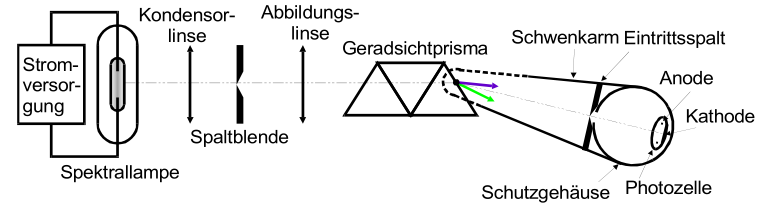
\includegraphics[width = 0.5\textwidth]{data/optischerTeil.png}
    \caption{Schematischer Aufbau des Versuches \cite{Anleitung500}.}
    \label{fig:aufbauOptik}
\end{figure}

\noindent
Durch den Strahlengang, den das Licht durchzulaufen hat, wird es gebündelt und durch das Geradsichtprisma in verschiedene Wellenlängen aufgespaltet, sodass
die Photozelle mit monochromatischem Licht bestrahlt wird. Der prinzipielle Aufbau der Photozelle, der Teil des Versuchaufbaus, in dem der eigentliche Photoeffekt
stattfindet, ist in \autoref{fig:photozell} abgebildet. In der Photozelle befinden sich zwei Elektroden, die auf der Innenseite 
mit einer Metalllegierung bedampft sind. Der Glaskolben ist evakuiert, sodass die Elektronen nicht mit Gasmolekülen wechselwirken.
\begin{figure}[H]
    \centering
    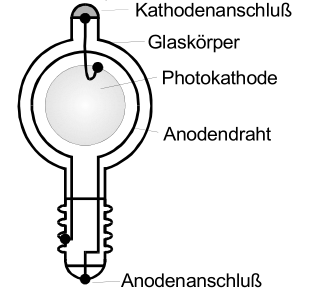
\includegraphics{data/photozelle.png}
    \caption{Schematische Darstellung der verwendeten Photozelle \cite{Anleitung500}.}
    \label{fig:photozell}
\end{figure}

\noindent
Zuerst wird für fünf verschieden Farben aus dem Spektrum, welches in \autoref{fig:spektrum} abgebildet ist, der Photostrom $I_{\text{Ph}}$ in Abhängigkeit der
Bremsspannung $U_{\text{Br}}$ gemessen.
\begin{figure}[H]
    \centering
    \includegraphics[width = 0.75\textwidth]{data/spektrum.png}
    \caption{Farbspektrum des Lichtes.}
    \label{fig:spektrum}
\end{figure}

\noindent
In einem zweiten Versuchsschritt wird das gelbe Licht mit einer Wellenlänge von $\SI{579}{\nano\metre}$ näher untersucht. Dafür wird eine Beschleunigungsspannung
angelegt und schrittweise um $\SI{1}{\volt}$ verringert. Gemessen wird in einem Bereich von $\SIrange{20}{-20}{\volt}$.